\documentclass[String-lecture-21.tex]{subfiles}


\begin{document}\section{Motivation and Overview}\label{sec:motivation}

\subsection{Why do we study string theory?}

$\bullet$ \textbf{For quantum gravity}


One of the major problems in theoretical physics is to provide a unified description of all the forces in Nature. The standard model has unified electromagnetic, weak and strong force based on quantum field theories whereas general relativity for gravity is formulated within classical physics. A quantum theory of gravity is needed to reconcile general relativity with the principles of quantum mechanics. However, it is known that the renormalization procedure does not cure ultraviolet divergence for gravity. Therefore, naive quantization of general relativity does not give a consistent theory.

String theory not only yields the first quantization of gravity but also resolves the renormalization problem of gravity by replacing point particles by vibrating strings.  To our knowledge, string theory is currently the only theory that has this property. Once we discover a candidate to unify gravity and quantum mechanics of all the forces, it is inevitable to try to understand it as well as we can although there is never any guarantee we can achieve.

Indeed, string theory has given deep insights into quantum gravity. The Beckenstein-Hawking formula \cite{Bekenstein:1973ur,Bardeen:1973gs,Hawking:1974sw} was microscopically derived by counting D-brane states with fixed mass and charge for certain (called extremal) black holes in string theory \cite{Strominger:1996sh}. The AdS/CFT correspondence \cite{Maldacena:1997re} conjectures that non-perturbative definition of string theory on AdS background is described by conformal field theory, and it partially resolves Hawking information paradox of black hole \cite{Hawking:1976ra}. Interestingly, a generalization of the Beckenstein-Hawking formula called the Ryu-Takayanagi entanglement entropy formula \cite{Ryu:2006bv}, connects quantum gravity and quantum information theory, which is actively studied in recent years. These developments certainly pose questions to basic concepts of spacetime.





\vspace{.3cm}




\noindent$\bullet$ \textbf{Rich arena for physics theories}


String theory has shed light on the behavior of an established physical theory. These range from proof of positive energy, quark confinement, heavy-ion collisions, quantum critical behavior, quantum black holes, quantum information, etc. Moreover, it sometimes sets up a new framework to study established physical theory. In my opinion, there are two reasons for it. One reason is that string theory can generate vast families (in fact, infinitely many) of quantum field theories in various dimensions. There are five types of string theories, Type I, IIA, IIB, Heterotic $\SO(32)$, $E_8\times E_8$ and M-theory is a limit of large dilaton expectation value in Type IIA  string theory. Also, Type II theories can contain D$p$-branes, and M-theory can have M2 and M5-branes. Although there are finitely many string theories, they can ``engineer'' infinitely many quantum field theories depending on manifolds string theory lives and brane configurations. The other reason is duality, equivalence between two different descriptions at quantum level. In fact, string theories of five types are related by a web of dualities (see the figure in the front page). The AdS/CFT correspondence is another kind of duality. More dualities have been (and surely will be) discovered in string theories, and a duality plays a crucial role in showing drastically different viewpoints for an established physical theory.

Through recent developments in string theory, especially in the study of M5-branes, we have learned that there are vast families of QFTs which do not admit Lagrangian description. They are intrinsically strongly-coupled so that techniques in QFT we have developed for decades cannot be used. Currently, we are trying to understand QFTs without Lagrangian description case by case by using dualities, dimensional reduction on some manifolds,  RG flows or perturbing theories. However, there is no consistent unified description for these theories. Therefore, we need a new framework to describe QFTs without Lagrangian description.


%
%There are many instances where questions are asked in the context of the established physical theory. They are often questions about known but intractable equations the standard physical theories where re-asking these questions in light of string theory has given us a lot more insights about the answers.

\vspace{.3cm}
\noindent$\bullet$ \textbf{For mathematical structure}

A certain group of people is interested in string theory because it has brought about a lot of new insights in mathematics, especially in geometry. String theory has repeatedly provided new ways to look at geometry, which arise as inevitable consequences of understanding how physical theory should be. Mirror symmetry \cite{Candelas:1990rm}, Seiberg-Witten invariants \cite{Witten:1994cg}, AGT relation \cite{Alday:2009aq}, etc are salient examples. Moreover, string dualities have led to highly non-trivial conjectures that connect seemingly different subjects of mathematics.  String theory provides many insights into geometry partly because we do not understand the theory.
In contrast to the fact that Einstein's theory of gravity has been constructed based on Riemannian geometry, we do not understand the geometric foundation for string theory yet.  However, physicists can develop new insights into geometry because physicists stumble upon a profound theory we do not understand well. There are certainly more mathematical secrets in string theory.


\vspace{.3cm}
\noindent$\bullet$ \textbf{Because we do not know what it is}

As mentioned, we do not understand the core new concept string theory is based on, but we know it is remarkably rich.
One reason that string theory is an exciting topic to work on for students is that so many things are not understood yet. It sometimes framed criticisms that string theorists do not understand the theory. That is true. However, if we understood it, there would be ground-breaking insights both in physics and mathematics. The fact that so little is understood and such relatively small pieces are actually such big discoveries in their own right makes us excited. Of course, there is still a lot more to do!

\subsection{Very very brief history}

String theory was invented originally by accident in trying to solve a different problem, subsequently developed by a long and fortunate process of tinkering. Therefore, the history of string theory itself is interesting. For detailed history of string theory, we refer to \cite{Greene:1999kj,Schwarz,Schwarz:2011ona,cappelli2012birth,Ooguribook,Polchinski:2017vik}.

String theory was first developed by aiming at describing hadron physics. People came up with the idea that a meson is a little string with charges at its end and the meson resonances are vibrational states of the string. Although this physical picture, which first emerged from the Veneziano amplitude \cite{Veneziano:1968yb}, is now believed to be qualitatively correct at a description of strongly interacting particles, QCD became far more successful in describing details of strong interactions soon later.

However, a small group of physicists continued to study string theory in the 70s, and it was found that string theory includes massless spin-two particles, suggesting that string theory can be a theory of gravity. Furthermore, a tachyon present in bosonic string theory turned out to be absent by incorporating supersymmetry, and Type IIA and IIB as well as Type I theories have been constructed.

In 1984, Green and Schwarz showed \cite{Green:1984sg} that anomaly pointed out by Alvarez-Gaum\'e  and Witten is canceled if the gauge group of Type I string theory is $\SO(32)$, which led to the first string revolution. A number of people have started working in the field of string theory. During the first revolution, Heterotic string theory was constructed.

In 1995, Witten proposed \cite{Witten:1995ex}  that dualities relate five types of string theories and they are moreover five different limits of one bigger theory called M-theory. This has led to the second string revolution during which D-branes are proposed and non-perturbative aspects of string theories have been extensively studied. These results bore fruits as discoveries of a number of dualities, understanding of quantum nature of black holes and the AdS/CFT correspondence.

The second revolution has driven more researchers to study D-brane world-volume theories and their relations to quantum gravity. However, dynamics on M2-branes and M5-branes that are fundamental degrees of freedom in M-theory have remained elusive. Triggered by the work of Bagger-Lambert \cite{Bagger:2006sk}, the world-volume theory for M2-branes was found to be a highly supersymmetric exquisite mixture of Chern-Simons gauge theory with some scalars and spinors \cite{Aharony:2008ug}. On the other hand, the world-volume theory on M5-branes is difficult to analyze because it is known that it does not admit Lagrangian description. However, the paper of Gaiotto \cite{Gaiotto:2009we} has ignited the study of properties of M5-branes by wrapping them on a certain manifold, which continues to be active so far.

The following picture shows the timeline of string theory and when the standard textbooks were written.\footnote{Of course, there are many other books \cite{Zwiebach:2004tj,johnson2006d,Dine:2007zp,Ibanez:2012zz,Blumenhagen:2013fgp,kiritsis2019string,tomasiello2022geometry} and notes \cite{Uranga,Tong:2009np,wray2011introduction,Hosomichi,Weigand}.} Obviously, the textbooks do not cover developments after their publications. We will mainly use Polchinski's textbook \cite{Polchinski}. However, I do not recommend you stick to only one book when you study a subject. Some parts are explained very well in a book, but some parts are sometimes hard to grasp for some people. Therefore, it is always a good idea to look for books, notes, and papers that suit you best.
\begin{figure}[ht]\centering
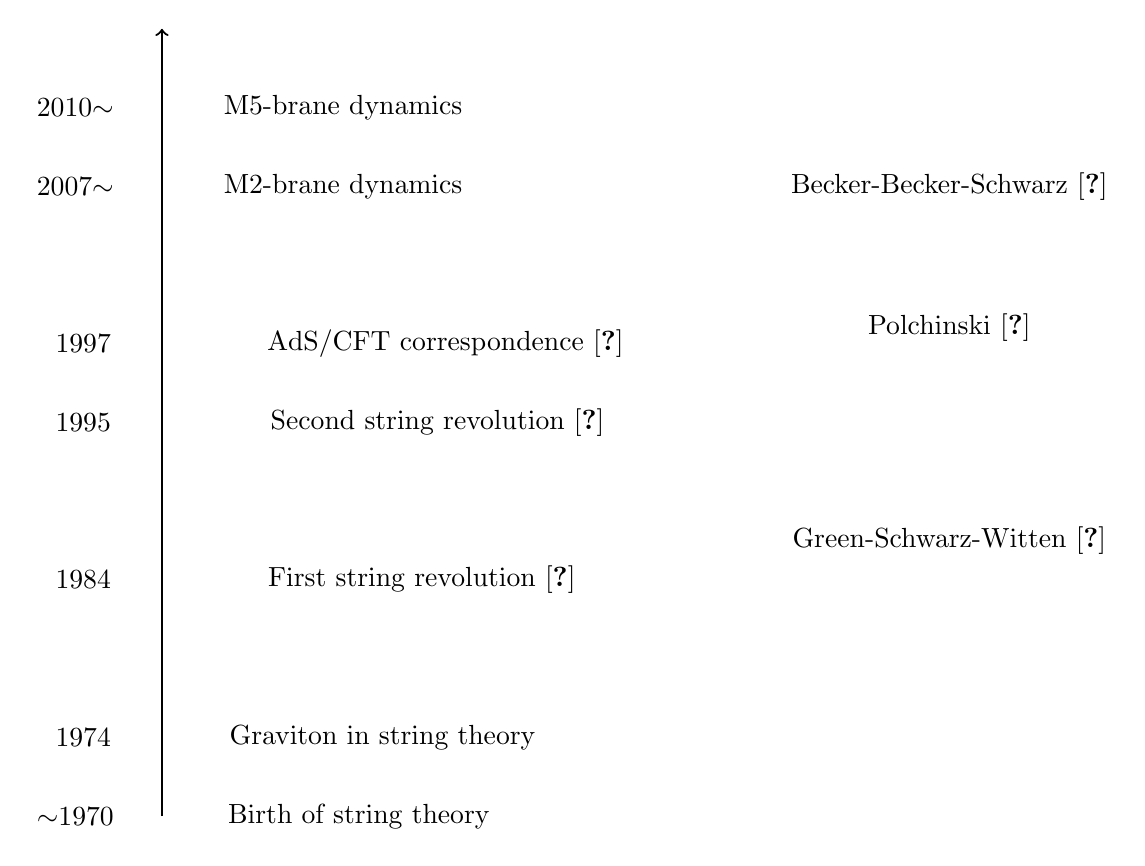
\begin{tikzpicture}
\draw[->,thick]  (0,0) to (0,10);
\node at  (2.3,9) {M5-brane dynamics};
\node at  (-1.1,9) {2010$\sim$};
\node at  (10,8) {Becker-Becker-Schwarz \cite{BBS}};
\node at  (2.3,8) {M2-brane dynamics};
\node at  (-1.1,8) {2007$\sim$};
\node at  (10,6.2) {Polchinski \cite{Polchinski}};
\node at  (3.6,6) {AdS/CFT correspondence \cite{Maldacena:1997re}};
\node at  (-1,6) {1997};
\node at  (3.5,5) {Second string revolution \cite{Witten:1995ex}};
\node at  (-1,5) {1995};
\node at  (10,3.5) {Green-Schwarz-Witten \cite{GSW}};
\node at  (3.3,3) {First string revolution \cite{Green:1984sg}};
\node at  (-1,3) {1984};
\node at  (2.8,1) {Graviton in string theory};
\node at  (-1,1) {1974};
\node at  (2.5,0) {Birth of string theory};
\node at  (-1.1,0) {$\sim$1970};
\end{tikzpicture}
\caption{History of string theory and textbooks}
\end{figure}



\subsection{Very short highlights}


$\bullet$ The basic idea in string theory is that different elementary particles are all vibrational modes of a single type of string.  There are two types of strings, open and closed, and a trajectory of a string is called the \textbf{string world-sheet} which is parametrized by $(\sigma,\tau)$.
If the typical size $\ell_s$  of a string is smaller than the resolution that an accelerator can provide, we cannot see this in the experiment involving elementary particles.
$$
(\textrm{Planck scale})\  10^{-33}\;\textrm{cm}\le \ell_s\le 10^{-17}\;\textrm{cm} \  (\textrm{TeV scale})
$$
We often use the parameter
$$
\a'=\ell_s^2%/(2\pi)^2
$$
which is the only free parameter in string theory. As we will see, the couplings in string theory are expectation values of dynamical fields (so-called moduli) which take their value dynamically.
\begin{figure}[ht]\centering
\includegraphics[width=10cm]{picture/openclosedstring}
\end{figure}

\vspace{.3cm}
\noindent $\bullet$ Application of the quantization rules provides us with the Fock space of string excitations. In bosonic string, the massless modes include among others
$$
\begin{array}{c@{\quad }c@{\quad }c@{\quad }c}
\textrm{open string}: & A_\mu & \textrm{spin 1}& \textrm{W-boson}\cr
\textrm{closed string}: & g_{\mu\nu} & \textrm{spin 2}& \textrm{graviton}
\end{array}
$$
In addition, one finds a tower of massive string excitations of mass
\begin{align}
\textrm{open bosonic}: &\quad M^2= \frac{1}{\a'} (N-1) \quad  \cr
\textrm{closed bosonic}: &\quad  M^2 = \frac{4}{\a'} (N-1)  \quad N = 0,1,2,\ldots \nonumber
\end{align}
Note that the lowest-lying state has a dimension of negative [mass]${}^2$ $(N=0)$, which is called \textbf{tachyon}. The bosonic theory is consistent only when the number of spacetime dimensions is 26. We can also refer to \cite{witten2018every}.



\vspace{.3cm}
\noindent $\bullet$ In the point-particle picture, the divergence appears when all four vertices come close to each other. On the other hand, the string word-sheet has no vertices. Thus, when we sum over all surfaces, we do not encounter configuration analogous to collapsed vertices. String theory amplitudes have no ultraviolet (shot distance) divergence.  As a result, string theory provides a finite quantum theory of gravity. Moreover, this is even better than renormalizable quantum field theories since there is no divergence in the first place.
\begin{figure}[ht]\centering
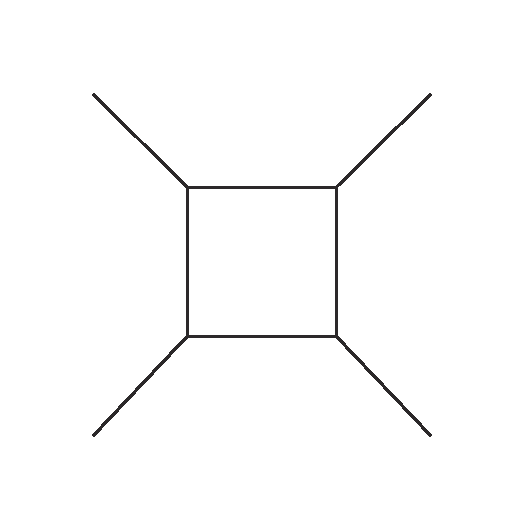
\includegraphics[width=4cm]{picture/Divergence} \hspace{2cm}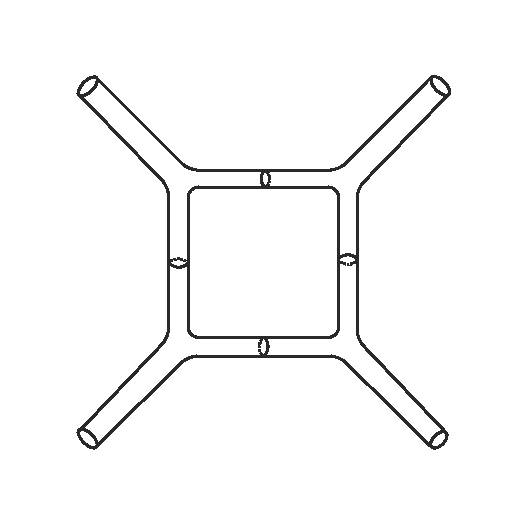
\includegraphics[width=4cm]{picture/String-loop}
\end{figure}




\vspace{.3cm}
\noindent $\bullet$
Strings, besides vibrating in usual spacetime, can also have some internal degrees of freedom. These internal degrees of freedom are fermionic. This can be quantized in a similar manner to that for bosonic strings. Then, a superstring can be considered as a string with symmetry between bosonic states and fermionic states. In superstring theories, the good features (e.g. emergence of gravity and UV finiteness) are preserved, and one can incorporate fermions. Moreover, as mentioned,  the tachyonic mode is absent.
\begin{enumerate}
\item the theory is consistent in 10 spacetime dimensions.
\item there are five fully consistent string theories in $d=10$.

Type IIA, Type IIB, Type I (open+closed string), $E_8\times E_8$ Heterotic, $\SO(32)$ Heterotic

\item Type II theories can have D-branes that accommodate open strings. Type IIA (resp. IIB) has D$p$-branes where $p$ is even (resp. odd), and Type I does D9, D5, D1-branes.


\item Furthermore, all the five apparently different string theories are different limits of the same underlying theory called  M-theory

\item In the low energy scale $\ll1/ \ell_s$, a theory is described by supergravity which combines supersymmetry and general relativity.

\end{enumerate}




\vspace{.3cm}
\noindent $\bullet$  How do we reduce the number of dimensions from 10 to 4? The answer is Kaluza-Klein mechanism/compactification.
If we take the 10-dimensional space of the form $\bR^{1,3}\times M$ where $M$ is a 6-dimensional compact space and its size is much smaller than the resolution of the most powerful accelerator $\sim 10^{-17}$cm, then a (9+1)-dimensional theory looks like (3+1)-dimensional.  In fact, in order for a theory to be consistent, $M$ has to be a Calabi-Yau manifold (which is endowed with a Ricci-flat metric). More importantly, the extra dimensions give ``room'' to derive the complexity of the real world from a simple setting.





\subsection{Convention}
% \SN{Summarize convention}

% In this lecture note, we use $\alpha'$ rather than string tension $T = \frac{1}{2\pi\alpha'}$. \SN{Do we need this comment?}
The world-sheet coordinate indices are denoted by the alphabet letter  $a, b,\ldots$, and the target-space coordinate indices are denoted by the Greek letter $\mu,\nu,\ldots$.

The world-sheet metric is denoted by $h_{ab}$.



\subsubsection*{spacetime}
In anticipation of
string theory, we consider $D$-dimensional Minkowski space
${\bR}^{1,D-1}$. Throughout
these notes, we work with signature
%
$$ \eta_{\mu\nu} = {\rm diag}(-1,+1,+1,\ldots,+1)$$
%

\subsubsection*{World-sheet}

We use $\sigma^a$ for a local coordinate of the world-sheet and we denote the metric by $h_{ab}$ in this local coordinate so that the measure is $\sqrt{h}d^2\sigma$ for a curved world-sheet.

We often consider the case that the world-sheet is topologically a cylinder or a plane.
The Minkowski cylindrical coordinates are denoted by $(\tau,\sigma)$ and the Euclidean cylindrical coordinates $(t,\sigma)$ where the Wick rotation is performed as $\tau=-it$. In the Euclidean coordinate, we introduce the holomorphic complex coordinate $w=it+\sigma$ for the cylinder. The conformal map brings the cylindrical coordinate to the plane coordinate by $z=e^{-iw}$.
\begin{itemize}
  \item right-moving or holomorphic coordinate: $\sigma^-=\tau-\sigma$ (Minkowski cylinder), $w=it+\sigma$ (Euclidean cylinder), $z$ (Euclidean plane),
\item  left-moving or anti-holomorphic coordinate: $\sigma^+=\tau+\sigma$ (Minkowski cylinder), $\overline w=-it+\sigma$ (Euclidean cylinder), $\overline z$ (Euclidean plane),
\end{itemize}

In the plane coordinate, the holomorphic coordinates are given by
  \begin{align}\nonumber
   z = \sigma^1 +i\sigma^2 \ , &\qquad  \ol z = \sigma^1 -i\sigma^2 \ \cr
   \partial \equiv \partial_z = \frac{\partial}{\partial z} = \frac{1}{2} \left( \partial_1 -i\partial_2 \right) \ , & \qquad
   \ol\partial \equiv \partial_{\ol z} = \frac{\partial}{\partial \ol z} = \frac{1}{2} \left( \partial_1 +i\partial_2 \right) \ ,
  \end{align}
The metric is given by
  \begin{align}\nonumber
   d^2z = dzd\ol z = 2 d \sigma^1 d \sigma^2  \ ,
  \end{align}
       where the factor $2$ comes from the Jacobian.
       One can also write
  \begin{align}\nonumber
   h_{z\ol z} = h_{\ol z z} = \frac{1}{2} \ , \quad h_{z z} = h_{\ol z\ol z} = 0 \ , \quad
   h^{z\ol z} = h^{\ol z z} = 2 \ , \quad h^{z z} = h^{\ol z\ol z} = 0 \ .
  \end{align}

\subsubsection*{Parameters and constants}
\begin{itemize}
  \item String theory has only one parameter $\alpha'$, and string length and tension are written as
\be
\ell_s=\sqrt{\alpha'}~, \qquad T=\frac{1}{2\pi\alpha'}
\ee
  \item String coupling is given by an expectation value $g_s=e^\Phi$  of the Dilaton field
  \item Planck length
  \be
  \ell_P=\sqrt{\frac{\hbar G}{c^{3}}}~, \qquad \ell_P^3=g_s\ell_s^3
  \ee
\item Coupling constants of $D=11$ and $D=10$ supergravities
\be
\frac{1}{2 \kappa_{11}^{2}}=\frac{2 \pi}{\left(2 \pi \ell_{p}\right)^{9}}~,\qquad \frac{1}{2\kappa_{10}^2} = \frac{2\pi}{(2\pi \ell_s)^8}
\ee
\end{itemize}


\subsection*{Acknowledgments and disclaimer}
We would like to express gratitude to students at Fudan University who have participated in the lecture series in 2017 and 2021 for providing useful comments on the note. In particular, we are grateful to Jiaqi Guo and Jack Yang for helping us to draw figures. We also thank Y. Tachikawa for informing \cite{cappelli2012birth} of the historical account.
The literature in string theory is too vast to be cited in full, and we are not entitled to accurately acknowledge historical developments of string theory. Therefore, we would like to delegate finding original literature to the reader. As mentioned above, there are already many good books on string theory, and this note covers only a small part of string theory. Nevertheless, we would be delighted if this note becomes a concise introduction to the huge subject for students.



\end{document}
